\documentclass[12pt, a4paper]{report}


\usepackage[T1]{fontenc}
\usepackage[latin1]{inputenc}
\usepackage[english]{babel}
\usepackage{siunitx}
\usepackage{graphicx}
\usepackage{tipa} % for the \ark{} command
\usepackage{graphics} % for pdf, bitmapped graphics files
\usepackage{times} % assumes new font selection scheme installed
\usepackage{amsmath}
\usepackage{latexsym}
\usepackage{amscd}% for commutative diagrams
\usepackage{mathrsfs} %this package is for the script font \mathscr
\usepackage{relsize}
\usepackage{delarray}
\usepackage{pstricks}
\usepackage{theorem}
\usepackage{changepage}
\usepackage{euscript}
\usepackage{textcomp}
\usepackage{esvect}
\usepackage{parskip}
\usepackage{placeins}
\usepackage{subfigure}
% \usepackage{subcaption}
\usepackage{array}
\usepackage{delarray}
\usepackage{stmaryrd}
\usepackage{fancyhdr}
\usepackage{graphpap}
\usepackage{makeidx}
\usepackage{enumerate}
\usepackage{esint}
\usepackage{datetime}
\usepackage{caption}
\usepackage{smartdiagram}
\usesmartdiagramlibrary{additions}
%Set Abstract Page
\usepackage{abstract}
\setlength{\absleftindent}{-5mm}
\setlength{\absrightindent}{-5mm}

%Colour definitions - put before TikZ
\usepackage{color}
\definecolor{igreen}{rgb}{0.0, 0.56, 0.0}
\usepackage{xcolor, colortbl}
\colorlet{gred}{-red!75!green!65!}
\colorlet{mamber}{-red!75!green!15!blue!50!}
\colorlet{grown}{-red!75!blue!20!green}
\colorlet{bled}{-red!85!blue!40!green!45!}
\colorlet{waters}{cyan!25} % Define color for the water
\colorlet{water}{cyan!25!green!20!} % Define color for the water
\definecolor{grin}{HTML}{00F9DE}
\usepackage{rotating}
\providecommand{\keywords}[1]{\textbf{\textit{Keywords---}} #1}

% For faint dotted table line
\usepackage{arydshln}
\setlength{\dashlinedash}{.4pt}
\setlength{\dashlinegap}{.8pt}

\usepackage{booktabs}
\usepackage{graphicx}
\usepackage{tikz}
\usepackage{tikz-3dplot}
\usetikzlibrary{
arrows,
arrows.meta,
automata,
backgrounds,
calc,
decorations,
decorations.pathmorphing,
decorations.pathreplacing,
decorations.fractals,
external,
fit,
matrix,
petri,
positioning,
shadows,
shapes,
shapes.multipart,
topaths,
intersections
}
\usepackage{eso-pic}
\def\ba{\begin{array}}
\def\ea{\end{array}}
\def\beann{\begin{eqnarray*}}
\def\eeann{\end{eqnarray*}}
\def\bea{\begin{eqnarray}}
\def\eea{\end{eqnarray}}
\def\bsy{\boldsymbol}
\def\gray#1{{\color{gray}#1}}

%% COUNTERS
\setcounter{MaxMatrixCols}{20}
\renewcommand{\thesection}{\arabic{section}}
\renewcommand{\thesection}{\thechapter.\number\numexpr\value{section}}
\renewcommand{\thesubsection}{\thesection.\number\numexpr\value{subsection}}
%%For changemargin
\def\quote{\list{}{\rightmargin\leftmargin}\item[]}
\let\endquote=\endlist 
\def\changemargin#1#2{\list{}{\rightmargin#2\leftmargin#1}\item[]}
\let\endchangemargin=\endlist 
\makeatletter
\newlength\qvec@height
\newlength\qvec@depth
\newlength\qvec@width
\newcommand{\qvec}[2][]{
    \settoheight{\qvec@height}{$#2$}
    \settodepth{\qvec@depth}{$#2$}
    \settowidth{\qvec@width}{$#2$}
  \def\qvec@arg{#1}
  \raisebox{.2ex}{\raisebox{\qvec@height}{\rlap{% 
    \kern.05em
    \begin{tikzpicture}[scale=1,shorten >=-3pt,shorten <=-3pt]
    \pgfsetroundcap
    \coordinate (Stx) at (.05em,0) ;
		\coordinate (Arx) at (\qvec@width-.05em,0) ;
    \draw[->](Stx) to[bend left] (Arx);
    \end{tikzpicture}
  }}}
  #2
}
\makeatother
\makeatletter
\newlength\pvec@height
\newlength\pvec@depth
\newlength\pvec@width
\newcommand{\pvec}[2][]{
    \settoheight{\pvec@height}{$#2$}
    \settodepth{\pvec@depth}{$#2$}
    \settowidth{\pvec@width}{$#2$}
  \def\pvec@arg{#1}
  \raisebox{.2ex}{\raisebox{\pvec@height}{\rlap{% 
    \kern.05em
    \begin{tikzpicture}[scale=1,shorten >=-3pt,shorten <=-3pt]
    \pgfsetroundcap
    \coordinate (Stx) at (.05em,0) ;
		\coordinate (Arx) at (\pvec@width-.05em,0) ;
    \draw[->](Stx) to[bend right] (Arx);
    \end{tikzpicture}
  }}}
  #2
}
\makeatother
\makeatletter
\newlength\vvec@height%
\newlength\vvec@depth%
\newlength\vvec@width%
\newcommand{\vvec}[2][]{%
  \ifmmode%
    \settoheight{\vvec@height}{$#2$}%
    \settodepth{\vvec@depth}{$#2$}%
    \settowidth{\vvec@width}{$#2$}%
  \else 
    \settoheight{\vvec@height}{#2}%
    \settodepth{\vvec@depth}{#2}%
    \settowidth{\vvec@width}{#2}%
  \fi%
  \def\vvec@arg{#1}%
  \def\vvec@dd{:}%
  \def\vvec@d{.}%
  \raisebox{.2ex}{\raisebox{\vvec@height}{\rlap{%
    \kern.05em%
    \begin{tikzpicture}[scale=1]
    \pgfsetroundcap
    \draw (.05em,0)--(\vvec@width-.05em,0);
    \draw (\vvec@width-.05em,0)--(\vvec@width-.15em, .075em);
    \draw (\vvec@width-.05em,0)--(\vvec@width-.15em,-.075em);
    \ifx\vvec@arg\vvec@d%
      \fill(\vvec@width*.45,.5ex) circle (.5pt);%
    \else\ifx\vvec@arg\vvec@dd%
      \fill(\vvec@width*.30,.5ex) circle (.5pt);%
      \fill(\vvec@width*.65,.5ex) circle (.5pt);%
    \fi\fi%
    \end{tikzpicture}%
  }}}%
  #2%
}
\makeatother
\def\ba{\begin{array}}
\def\ea{\end{array}}
\def\beann{\begin{eqnarray*}}
\def\eeann{\end{eqnarray*}}
\def\bea{\begin{eqnarray}}
\def\eea{\end{eqnarray}}
\def\bsy{\boldsymbol}
\def\gray#1{{\color{gray}#1}}
\usepackage{titlesec}
\usepackage{multirow}
%To reference within text
\usepackage{hyperref}
\usepackage{apacite}
\usepackage{lipsum}
\usepackage{tikz-cd}
\usepackage{float}
\usepackage{titling}
\usepackage{epigraph}
\usepackage[title, titletoc]{appendix}
\setlength\epigraphwidth{8cm}
\setlength\epigraphrule{0pt}

\titleformat{\chapter}{\normalfont\LARGE}{\thechapter\,$\vert$}{20pt}{\LARGE}{\setcounter{chapter}{0}}
\setlength{\headheight}{15pt}
\titlespacing*{\chapter}{0pt}{-70pt}{40pt} %Move chapter titles up
% Title page logos:
\makeatletter
\newcommand\BackgroundPicturea[3]{
	\setlength{\unitlength}{1pt}
	\put(0,\strip@pt\paperheight){
		\parbox[t]{\paperwidth}{
			\vspace{#2}\hspace{#3}
			\mbox{\includegraphics[scale=0.5]{#1}}
}}}
\newcommand\BackgroundPictureb[3]{
	\setlength{\unitlength}{1pt}
	\put(0,\strip@pt\paperheight){
		\parbox[t]{\paperwidth}{
			\vspace{#2}\hspace{#3}
			\mbox{\includegraphics[scale=0.3]{#1}}
}}}
\makeatother
% For my abbreviations
\newcommand{\abbrlabel}[1]{\makebox[3cm][l]{\textbf{#1}\ \dotfill}}
\newenvironment{abbreviations}{\begin{list}{}{\renewcommand{\makelabel}{\abbrlabel}}}{\end{list}}
% Line Spacing
\usepackage{setspace}
\setstretch{1.5}
%Set of command is for the changemargin environment
\def\quote{\list{}{\rightmargin\leftmargin}\item[]}
\let\endquote=\endlist 
\def\changemargin#1#2{\list{}{\rightmargin#2\leftmargin#1}\item[]}
\let\endchangemargin=\endlist
%Replace Contents to Table of Contents	
\addto\captionsenglish{
	\renewcommand{\contentsname}%
	{Table of Contents}
	\setcounter{tocdepth}{3}% Include \subsubsection in ToC
	\setcounter{secnumdepth}{3}% Number \subsubsection in ToC
	}
\renewcommand{\listfigurename}{List of Figures}
\renewcommand{\listtablename}{List of Tables}


\theoremstyle{definition}
\newtheorem{definition}{Definition}[section]
\newtheorem{proof}{Proof}[section]

\newtheorem{theorem}{Theorem}

\hypersetup{pdftitle = Project Report, pdfauthor = {First Last}, pdfstartview=FitH, pdfkeywords = essay, pdfpagemode=FullScreen, colorlinks, anchorcolor = red, citecolor = blue, urlcolor=blue, filecolor=green, linkcolor=red, plainpages=false}
%%%%%%%%%%%%%%%%%%%%%%%%%%%%%%%%%%%%%%%%%%%%%%%%%%%%%%%%%%%%%%%%%%%%%%%
\pagestyle{fancy}
\rhead{Christ Church}
\chead{}
\lhead{University of Oxford}
\lfoot{\date{}}
\cfoot{}
\rfoot{\thepage}
% Top and Bottom Line Rules
\renewcommand{\headrulewidth}{0.4pt} %0.4pt
\renewcommand{\footrulewidth}{0.4pt}
\fancyheadoffset{9pt}
\fancyfootoffset{9pt}
% Line spacing
\renewcommand{\baselinestretch}{1.5} %1.5
%%%%%%%%%%%%%%%%%%%%%%%%%%%%%%%%%%%%%%%%%%%%%%%%%%%%%%%%%%%%%%%%%%%%%%%
\date{}

\title{Active Learning}
\author{\\ \Large{John Ryan}
\\ Christ Church
\\
\\
\\
\\ University of Oxford
\\
\\ \\
Trinity 2021
}
%%%%%%%%%%%%%%%%%%%%%%%%%%%%%%%%%%%%%%%%%%%%%%%%%%%%%%%%%%%%%%%%%%%%%%%

\DeclareMathOperator{\E}{\mathbb{E}}

\begin{document}
% Adjust logo positions here
\AddToShipoutPicture*{\BackgroundPicturea{Logos/logo2.png}{0.7in}{5.8in}}

\thispagestyle{headings}
	\maketitle
\FloatBarrier
\pagenumbering{roman}


\thispagestyle{empty}
\begin{abstract}

Active Learning is an use

\keywords{Keyword1 - Keyword2 - Keyword3}
% \vspace{-10mm} %To remove added white space after
\end{abstract}
\tableofcontents
\thispagestyle{plain}
\listoffigures
\listoftables

\chapter*{List of Abbreviations}
\begin{abbreviations}
    \item[GP] Gaussian Process
    \item[GPC] Gaussian Process Classification
    \item[BALD] Bayesian Active Learning by Disagreement
    \item[ELBO] Evidence Lower Bound
    \item[ML] Machine Learning
\end{abbreviations}

\chapter{Introduction}
\pagenumbering{arabic}

Active learning is an area of machine learning where we are attempting to select which unlabelled datapoints we believe would be best to learn the label of. It is important because in many important use cases (for example, medical data), it is often either quite costly or just simply impossible to collect an incredibly large dataset. However current approaches to do it suffer from issues related to quality of aquired datapoints, model requirements and computational issues.

Bayesian ML models are the standard ways of building machine learning models which can calculate uncertainty well, however many of the standard approaches to doing so (MC Dropout) can give suboptimal performance, for example requiring a substantial amount of sampling. Gaussian Processes are a ML approach which give very good uncertainty performance, and new results in the field [DUE] have shown successful training of Variational Gaussian Processes with feature extractors and demonstrate that they maintain good uncertainty performance.

\section{Motivation}

Active Learning is an active area of Machine Learning where we are trying to select (unlabelled) data points in an attempt to maximise some objective.
\section{Aim and Objectives}

The aims of this report is to

\begin{itemize}
    \item Give an outline of the various methods for Active Learning which have been published
    \item Compare these methods in a reproducible and standardised fashion
    \item Extend and combine some of these approaches with other ML research to improve Active Learning performance in certain situations.
\end{itemize}
\section{Project Report Outline}
The remainder of this report is organised as follows:
\begin{itemize}
    \item[] \textbf{Chapter} \hyperref[Chap2]{\textbf{2}} --- Defines active learning, and introduces the different active learning methods from the literature.
    \item[] \textbf{Chapter} \hyperref[Chap4]{\textbf{4}} --- introduces Gaussian Process based models
    \item[] \textbf{Chapter} \hyperref[Chap5]{\textbf{5}} --- Combines BatchBALD and GPC
\end{itemize}
>

\chapter{Active Learning Methods}
\label{Chap2}

In a common active learning formulation we have the following setup.

\begin{itemize}
    \item $X_{pool}$ this is the distribution of the dataset which we have to work with in our data pool.
    \item $X_{true}$ this is the true real world distribution.
\end{itemize}

A common (and sensible) assumption is to assume that these distributions are the same.

Our machine learning models which we use to model a problem constrain the set of possible functions which we can represent and learn, this is how we imbue the problem with our prior beliefs about the nature of the problem.

- There are hard constraints (eg clipping the output of the model), which even given an unlimited amount of data our model can not possibly "learn around"
- There are softer constraints (priors over weights in a layer), which our model should be able to learn correctly given sufficient new data even if our prior is poor*.

This paramaterisaton of our models is very important, this is an assumption we are making about our problem.

An important observation is that the dataset we are using for training is (unless performing very simple active learning approaches eg random acquisition) not going to be the same as the true dataset which we are working with. 

This violates a very common assumption that we assume for convergence in many ML methods, and is something worth keeping in mind. This statistical bias is looked at in the following paper \cite{farquhar2021statistical}.

When working with Active Learning we are also normally working with much smaller datasets than is standard in ML, our models which are normally over paramatised to begin with become even more so, this can lead to training issues.

\section{Random}

The most straightforward acquisition function is to randomly sample from the poolset. This is a surprisingly strong baseline for for many datasets. For example with an unbalanced dataset random aquisition can fall behind as it will on average select points in the same proportion as which they occur in the pool. Here we have a comparision between unweighted MNIST and weighted MNIST with random aquisition.

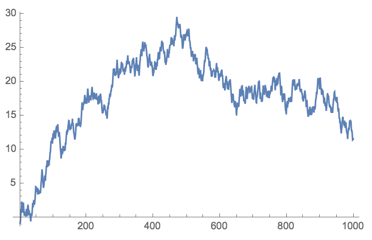
\includegraphics{todo}


\section{BALD}
Bayesian Active Learning by Disagreement (BALD) \cite{houlsby2011bayesian} is an active learning method which is based on selecting datapoints which maximise the mutual information between the datapoints class output and the models parameters. The paper details how we can instead of computing this in the paramater space which would be computationally prohibative in many cases, we can compute the same objective in the output space.

$${\arg\,\max}_x H \left[ \theta | D \right] - \mathbf{E}_{y \sim p(y | x, D)} \left[ H\left[ \theta | y, x, D\right]\right]$$

$${\arg\,\max}_x H \left[ y | x, D \right] - \mathbf{E}_{\theta \sim p(\theta | D)} \left[ H\left[ y | x, \theta \right]\right]$$


An issue which we run into when using BALD in the case where we want to select multiple datapoints to aquire at the same time is the fact that selecting the $n$ points with the greatest individual information content will not necessarily give you the $n$ points which jointly have the greatest information content. This can be made very obvious by considering the case when there is duplicates in the dataset. If the duplicated point is in the top n points as decieded by the BALD score, having both of the points in your aquired batch will give you no more information than just having one of them, you would be better served by selecting any other point instead of these points.

\section{BatchBALD}
BatchBALD \cite{kirsch2019batchbald}, is an extension of BALD designed especially to deal with the issues which we run into when using BALD to aquire batches of points.

To do this the objective function is modified, the original BALD objective is retained by setting $n = 1$ .

The BatchBALD score function is as follows.


\begin{definition}[BatchBALD]
    $$s_{BatchBald} (x_1, \ldots, x_n) = H(y_1, \ldots, y_n) - E_{p(f)}\left[H(y_1, \ldots, y_n | f)\right]$$
\end{definition}


\begin{definition}[Submodularity]
    A function $f : P(X) \rightarrow \mathbf{R}$ is sub modular if for all $A,B \subseteq X$ we have the following.

    $$f(A) + f(B) \geq f\left( A \cup B \right) +  f\left(A \cap B \right) $$
\end{definition}

The authors of the paper prove that the objective function that they specify is \textit{submodular}, which enables a greedy $1 - \epsilon$ approximation algorithm for selecting the optimium batch.



As the variables are independent conditioned on the value of the function, the right hand side of the equation factors into a sum over conditional expectations for each individual datapoint. The computationally difficult part of this objective is the computation of the joint entropy as this does not factor similarly. In fact, the summation required to compute this value is exponential in the number of datapoints we are currently considering. Estimating the entropy of a discrete distribution is something which we will investigate later \hyperref[sec:Entropy]{here}.


The authors of the paper address this issue by using sampling to estimate the joint entropy for larger batch sizes. The BatchBALD paper uses Bayesian Neural networks (BNNs) as their model. They are then able to sample from the weight distribution once to obtain a function draw for all possible inputs. This is not an ability we have when using GPCs, which we will come back to later.


\section{Joint Entropy}

We can also simply use the joint entropy alone as the active learning objective

$$s_{Entropy} (x_1, \ldots, x_n) = H(y_1, \ldots, y_n)$$

\begin{theorem}[$s_{Entropy}$ is submodular]
    Proof.
    Let $A_x,B_x \subseteq D_{pool}, C_x = A_x \cap B_x$
    
    $\hat{A} = A_y \setminus C_y, \hat{B} = B_y \setminus C_y$
    \begin{align*}
        s_{Entropy} (A_x) + s_{Entropy} (B_x) &= H(A_y) + H(B_y)\\
        &= H(C_y \cup \hat{A}) + H(C_y \cup \hat{B})\\
        &= H(\hat{A} | C_y) + H(\hat{B} | C_y) + 2 H(C_y)\\
        &\geq H(\hat{A}, \hat{B} | C_y) + 2 H(C_y)\\
        &= H(\hat{A}, \hat{B}, C_y) + H(C_y)\\
        &= H(A_y \cup B_y) + H(A_x \cap B_x)\\
        &= s_{Entropy} (A_x \cup B_x) + s_{Entropy} (A_x \cap B_x)
    \end{align*}

\end{theorem}

The fact that this objective is submodular enables us to use the same greedy $1 - \frac{1}{\epsilon}$ approximation algorithm as used above.

A justification for the use of this objective can be seem as attempting to minimise the entropy over the remaining items in the pool given the batch which we select.


$$\min_{B} H( \left(P \setminus B\right) | B) = \min_{B} H(P) - H(B) = \min_{B} - H(B) = \max_B H(B)$$

If we assume that the samples in the poolset are samples from the true distribuiton, we can view this as attempting to minimise the entropy of the output variables maximally fast, this is in contrast with the BALD objective which attempts to minimise the entropy of the paramaters maximially fast.

In the next chapter we will discuss some reasons while this may be preferable when using a Gaussian Process Classifer.

\chapter{Gaussian Process Based Models}
\label{Chap4}


\section{Gaussian Processes}


\begin{definition}[Gaussian Process]
    A Gaussian processes is a collection of random variables, any finite number of which have a joint Gaussian distribution. \cite[]{rasmussen2003gaussian}
\end{definition}


We can completely specify a Gaussian Process over a space $\chi$ by giving a mean function $m(\cdot), m : \chi \rightarrow R$, and covariance (kernel) function $k(\cdot, \cdot), k: \chi \times \chi \rightarrow R$.


For $k$ to be a valid covariance funciton we need for any evaluation of the covariance matrix to be a symetric positive definite matrix (as all covariance matrices of random variables must be S.P.D).

\begin{definition}[Positive Definte Matrix]
    A positive definite matrix is a matrix which has positive eiginvalues.
\end{definition}

\subsection{As distributions over functions}

We can view a Gaussian Processes as a distribution over functions. The space of functions which we can represent by a particular Gaussian Process is paramaterised by the kernel function which we are using.

We can understand this by investigating the interpretation of kernels as Repreducing Kernel Hilbert Spaces.





Gaussian Processes have a number of useful properties such as being closed under conditioning and marginalisation.

For the covariance function to define a valid MVN for all inputs the covariance function must be positive definite.

A positive definite kernel function can be represented by a feature space where the value of the kernel between 2 values can be computed by taking the inner product of the feature space of the 2 values.

Certain kernel functions such as the radial basis kernel, is represented by an infinite dimensional feature space. This infinite dimensional feature space enables it to model arbitarily complex functions. Polynomial or linear kernels do not enable this level of expressibility.

We can use Bayes rule to update the covariance and mean function from our prior, to the postior given noisy of exact data. The complexity of doing this (given arbitary kernels) is bounded by matrix inversion and  multiplication of a matrix of size of the number of datapoints in which we are using. The complexity of which is sub cubic, however in general the matrix multiplication algorithms we use practically are of the cubic variety).

This can be done as follows: 

(TODO) put update equations.

\subsection{Scaling to large data}

Unlike other methods we use often in machine learning, such as neural networks which have linear complexity in the size of the dataset we have superlinear complexity.

\subsubsection{Inducing Points}

In inducing point models, we instead of using all of the datapoints in our model. We instead use a smaller number of datapoints as an approximation to the true model. Various approaches exist for selecting the points we keep in our approximation.

One of the most sucessful approaches is to treat these inducing points as model parameters which we attempt to learn by minimising some objective.

Minimising the evidence lower bound (ELBO) is a common and principled object for this task.

Minimising this objective minimises the KL Divergence between the true output distribution and the approximate distribution we are learning.

\subsubsection{Random Fixed Features}

(Todo)





\section{Gaussian Process Classification}


To use Gaussian Processes for classification we have several issues to overcome.

The output of a Gaussian Process is a Multivariate Normal, this is a continous distribution over the real space, however in the classification setting we wish to have a categorical output. Which means we need to have a distribution over the the simplex.

We can in theory use any link function to convert a sample from our MVN in $R^n$ to a sample over the simplex, different link functions have different properties computationally and statistically.

\subsection{Link Functions}

The link function between the latent function (our GP) and the output of our classifier is again another parameter of the model.

\subsubsection{Logit}

The logit is the standard link function for the vast majority of GPC use cases. The use of the logit implicitly makes our GPC model obey the independence of irrelevant alternatives axiom from decision theory. 


$$p\left( y = k | f\right) = \frac{e^{f^T w_k}}{\sum_{i=1}^{K} e^{f^T w_i}}$$
\subsubsection{Probit}

The probit is a different link function which is normally defined for the binary classification case as the inverse of the CDF of a Gaussian. We can generalise this link function as follows.

$$p\left(y = k | f\right) = \mathbf{1}_{argmax_i(f_i) = k}$$


The probit function is easier to work with analitically, and great use of this is made in the binary classification case []. However it is clear from the defintions that a single sample draw from a GPC using a probit will not give an accurate assement of the confidence of the model. The computaion of the marginalisation of this objective over $f$ is investigated in \hyperref[sec:Integration]{later}.

\subsection{Minimising entropy over functions}

When using a softmax link function


\section{Training}

Using a straightforward Gaussian Process with no hyper parameters, for regression there is nothing to train. We simply have the exact equations to compute the posterior distribuiton at any possible input. In contrast to many optimization problems our output for any particular value is not a point estimate, it is a distribuiton so our objective should take this into account.


\subsection{KL Divergence}

\begin{definition}[KL Divergence (Entropy)]
    For 2 discrete probability distributions $P, Q$ defined on the same probability space $\aleph$
\end{definition}

\subsection{ELBO}

It is often quite difficult to compute the \textbf{KL Divergence}, as often we don't have direct access to one of the distribuitons which we are attempting to calculate it with.

The Evidence Lower Bound is a tractable objective which it is much easier for us to compute than the KL divergence and maximising this objective is equivalent to maximising the KL Divergence.

\begin{definition}[ELBO]
    
\end{definition}


\begin{proof}[Maximisng the ELBO will minimise the KL Divergence]
    \begin{align*}
        D_{KL} \left( Q || P \left(L | X\right) \right) &= 
    \end{align*}
\end{proof}


\chapter{vDUQ / DUE}

vDUQ / DUE \cite{vanamersfoort2020uncertainty} is a recent model which deals with some of the issues with using deep kernel learning with GPCs. DUE uses an inducing point GP to enable it to scale to large amounts of data.

This model is designed to have good uncertainty properties by enforcing sensitivity and bounding the amount by which any 2 inputs can diverge in the feature space. These properties are maintained by the additon of residual connections to the model and by performing spectral normalisation to bound the lipshitz constant of the layers in the feature extractor.

\section{Spectral Normalisation}

\begin{definition}[Lipshitz Constant]
    Given a function $f: X \rightarrow Y$, where $(X, d_x)$ and $(Y, d_y)$ are metric spaces. A lipshitz constant of the function $f$ is a value of $k$ such that.

    $$\frac{d_y(f(x_1), f(x_2))}{d_x(x_1, x_2)} \leq K, \forall x_1, x_2 \in X $$
\end{definition}

Some times we refer to \textit{the lipshitz constant} of a function, this is normally taken to mean the smallest value $k$ which is a lipshitz constant.

In our particular problem we are dealing with spaces in $\mathbf{R}^n$. The metric on this space which we will be using is the $L_2$ norm, (also known as the euclidean distance).

The lipschitz constant is a measure of how far apart 2 outputs to the function can be in terms of their inputs.

In the case where $f: R^n \rightarrow R^m$ and $f$ is a linear transformation we get a familar result.

\begin{align*}
    \min_k  \forall x_1,x_2 \in X \frac{d_y(f(x_1), f(x_2))}{d_x(x_1, x_2)} \leq K &= \min_k \forall x_1,x_2 \in X \frac{ L_2(Ax_1 - Ax_2)  }{ L_2(x_1, x_2)} \leq K \\
    &=  \min_k \forall x_1,x_2 \in X  \frac{ ||A(x_1 - x_2)||_2  }{ ||x_1- x_2||_2 } \leq K \\
    &=  \min_k \forall x \in X  \frac{ ||Ax||_2  }{ ||x||_2 } \leq K \\
\end{align*}

After the substitution we obtain an expression which from linear algebra we know is the matrix norm of $A$ induced by the vector norm which we have chosen, in this case the $L_2$ norm. The induced matrix norm by the $L_2$ vector norm has the nice property that it is the \textit{largest singular value} of the matrix which is also the square root of the largest eigenvalue.

For all of the linear layers in our model we now know how we can compute the respective lipschitz constants.

\begin{theorem}[Lipschitz constant of function compositions]
    If $lip(f) = a$ and $lip(g) = b$, then $lip(f \circ g) \leq a * b$
\end{theorem}

It turns out that the majority of activation functions which we use in our neural networks have a lipschitz constant of $\leq 1$, eg relu. This enables us to compute an upper bound of the lipschitz constant of our model by computing the lipschitz constant of all of the indiviudal layers and taking the product of those constants.



\subsection{Power Method}

Directly computing the largest singular value via computing the Singular Value Decompoisition of each linear transform is quite computationally prohibative, however there is a way in which we can approximate this value quite cheaply and accurately.

The \textbf{power method} is defined by a recurrence relation.

\begin{definition}[Power Method(for square matrices)]
    $$v_{k+1} = \frac{Av_k}{||Av_k||} $$
\end{definition}

This recurrence relation will converge if 2 conditions are met.

\begin{itemize}
    \item $A$ has a strictly largest eigenvalue
    \item $v_0$ has a non zero component in the direction of the largest eigenvalue
\end{itemize}

We compute the eigenvalue from the rayleigh quotent from our approximate maximum eigenvector. $\frac{v_k^T A v_k}{v_k ^ T v_k}$

If we chose a starting vector $v_0$ with uniform probability over all possible directions the second condition will be fullfilled with a probability of $1$.

The convergence ratio of this algorithm is $\frac{|\lambda_1|}{|\lambda_2|}$, so the convergence rate depends on the size of the second largest eigenvalue also.


To extend this to work with non square matrices we can either compute $A^TA$ or $AA^T$, use the power method to calculate its maximum eigenvalue and this is the spectral norm of $A$.
There is another approach which enables us to bypass this computation by instead of maintaining just 1 eignevector, we maintain a left and a right domainant eigenvector

\begin{definition}[Power Method(for non square matrices)]
    $$v_{k+1} = \frac{A^Tu_k}{||A^Tu_k||}, u_{k+1} = \frac{Av_k}{||Av_k||} $$
\end{definition}

Then with these appoximate eigenvectors we can approximate the singular value with $u^T A v$

To bound the lipschitz constant of a linear layer to a values, call this value $\sigma$. We can calculate the spectral norm $\alpha$, check if $\alpha > \sigma$. If this is true, we muliply the linear layer by $\frac{\sigma}{\alpha}$.

To maintain this during training we are required to compute this value during every forward pass. Due to the fact that given a sufficently small learning rate we expect that the change to linear layer will be small, if we use the previous forwards passes final vector(s) as our starting vector instead of randomly restarting we can greatly speed up the convergence of the recurrence relation. We find that empircally we can actually get very good performance with a single iteration of this method at each stage.


\section{Residual Connections}

Residual connections were introduced in by [cite]. One of their origianl 


\section{Modifications}

While DUE is an extremely powerful model, some modifications were required to help the performance and stability of the model when working with small amounts of data. 

\subsection{Natural Gradient Descent}

Natural Gradient Descent is an optimization method which is designed for when we are attempting to optimise some objective of a distribution. The use of this method greatly improved the rate of convergence and overall performance.


\begin{definition}[Gradient Descent]
    Gradient Descent is an iterative optimization algorithm where we modify the paramter in the direction which has the steepest gradient with respect to our objective function.
    $$p_{k+1} = p_{k} -  \alpha \nabla L(p_k)$$
\end{definition}

With a well chosen hyperparameter $\alpha$ and a convex loss function $L$ we can obtain convergence guarentees. [cite]. Many machine learning problems which we use gradient descent for do not obey the constraints which we require for guarentees of convergence [], empircally however the performance achieved by gradient descent and its derivates is impressive even these problems in many cases.

Instead of applying the gradient descent algorithm to the paramaters in the eucliedean geometry of the paramater space, instead we can use the geometry of the likelihood space paramaterised by our paramaters to enables superior optimization.

To create this method we will be attempting to minimise the KL Divergence between the distribuiton which we are paramaterising, and some objective distribuiton. We for example could be using the ELBO as defined previously in [].


We can take the taylor expansion of the objective below.

$$D_{KL} \left(p_\theta || p_{\theta+ \epsilon} \right) = $$




\begin{definition}[Natural Gradient Descent]
    
\end{definition}









\chapter{Combination}
\label{Chap5}

\section{Investigation of Exact Computation}

\label{sec:Integration}

If we use Probit as our link function the joint entropy can be computed exactly (unlike in the general case), however the complexity of this exact computation is very high.

To perform exact inference of the probit of a Gaussian Classifier we must perform integration of a Gaussian.

We wish to find the probability that a certain element of a MVN is the largest element. This corresponds to integrating the Gaussian over the subset of the space where this coordinate is the largest.

$$P(X_C > X_1 \land \ldots \land X_C > X_n) = \int_{x_c \in \{ -\infty, \infty \} } \ldots \int_{x_n \in \{ -\infty , x_c \}} p(x) dx$$

This can be interpreted as integrating on one side of several hyperplanes.

These planes are of the form $x_c = x_i$

With the linear transformation of $T = I - e_c 1^T$ we get to transform this integral.

$Z = TX$.

$Z \sim N(T \mu, T \Sigma T^T)$

We drop the original index (as we are marginalising over it) and it is degenerate. We could alternatively make T a projection into a c-1 dimensional subspace.

If we are doing this over multiple datapoints, we can transform each of the subsets of variables via the method above.

After performing this transformation we have a standard orthant integral which we can compute. Algorithms exist for computing this exactly in $O(p^2 2^p)$ using recursive integration and subspace projection. \cite{orthant}


However the number of dimensions which we are performing this integration over is (number of variables) * (number of categories - 1). With the exponential complexity this an infeasible method of computation.



\section{Sampling}

Given the difficultly of performing exact computation of the quantities required for the BatchBALD objective, the general approach is to use methods which rely on sampling.

In comparision with the approach performed in the BatchBALD paper where sampling is done over the weights of the Bayesian Neural Network, when we have a Gaussian Process as our output. It is not as straightforward to take a sample function from our postior. If we are to take a sample function output over a set out points, we would need to compute the joint distribution of these points and then take a sample from this distribution and pass this through our link function.
The complexity of performing this is cubic in the size of the pool, this complexity is unacceptably high as we are often working with quite large pool sizes.

This means that we can not use the same computational tricks used previously to speed up these calculations, however we can take advantage of other properties of Gaussian Processes to make some improvements in this aspect.


\section{Entropy}
\label{sec:Entropy}

\begin{definition}[Entropy]
    For a discrete r.v $X$ the entropy is defined as $$H(X) = - \sum_{x \in X} p(x) \log p(x) $$
\end{definition}


We require the ability to compute the joint entropy of a large number of random variables to compute several of the score functions which we are evaluating.

\subsection{Gaussian Process Classifer}
As we are using a Gaussian Process Classifier, the random variable of which we are trying to estimate the value of is of a known form.


$$ \mathbf{f} \sim N(\mu, \Sigma) $$
$$ \mathbf{p} =  \sigma \left(f \right) $$
$$ X_i \sim Cat(p_i) $$

The distribution $p(x)$ does not have a closed formula. We can estimate $p(x)$ via estimating the intergral via monte carlo intergration.

When we are considering larger and larger pool sizes the number of possible states of our random variable grows at an exponential rate.

With $C$ classes the entropy sumation will have $C^n$ terms in it. 

As we have that $ X_i \perp\!\!\!\perp X_j | f$, for a given likelihood sample we can store the exponential number of terms in a factored form. We for a sample $f$, we can compute $p(x_i = c | f)$ for each of the datapoints. To reconstruct the joint distribution for this function sample we take the product of the terms and relevant categories.


$$ p(X) = p(x_1, \ldots, x_n) = \E_{l \sim p(l)}  p(x_1, \ldots, x_n | l) = \E_{l \sim p(l)} \prod_{i=1}^n  p(x_i| l)$$

\subsection{Estimating the entroy}

The are 2 different approaches we can use in the estimation.

\subsection{Taking samples from the distribution}

We can take samples from the distribution, and then use these samples to estimate the entropy.



\subsubsection{Plugin Estimator}
The most straightforward approach is to use the \textit{plugin estimator}. This approach is to take $k$ samples from the distribution of interest, calculate the observed probability of each class and compute the entropy.

As we define the term in the entropy summation as $0$, when the probability is $0$. Using this approach bounds the number of terms in the summation by $k$.

$$p_j = \frac{1}{k} \sum_{i=1}^k \mathbf{1}_{X = j} $$

$$\hat{H}_k = - \sum_{i=1}^{c} \hat{p}_i \log{\hat{p}_i}$$


Some of the convergence properties of the plugin estimator are below.
$$\E \left(H - \hat{H}_k \right)^2 = O \left ( \frac{1}{k} \right) $$

$$ \frac{\sqrt{K}}{\sigma} \left(H - \hat{H}_k \right) \sim \mathbf{N} \left(0, 1 \right) $$



\subsubsection{LP Estimator}

Using an \textit{LP Estimator} [cite] we can estimate the the entropy with far less samples in comparision to using a plugin estimator. The required number of samples from the distribution to estimate the entropy well is \textit{sublinear}, of the order $O \left( \frac{d}{\log{d}}\right)$, where $d$ is the number of values in the domain which have positive support. However the amount of values with support in our problem is going to be exponential as our final layer is a softmax, which means that $d = c^n$.


\subsection{Sampling from the outer summation}

As we can actually compute the values $p(x)$ without sampling from the final categorical distribution, we can take advantage of this fact to improve the performance of our estimator. We can directly obtain the probabilities after the softmax. This enables us to perform the estimation in 2 steps.

\begin{itemize}
    \item Sample from the outer summation to see which values of $p(x)$ we are required to compute.
    \item Estimate $p(x)$ directly from the output of the softmax.
\end{itemize}

We can also take advantage of the fact that the output variables are conditionally independent given a function sample. This enables us to sample from $p(x)$ without requiring an exponential amount of computation by sampling from the distribution in the following the following sequence of steps.

\begin{itemize}
    \item Sample from the likelihood distribution $p(l)$
    \item Put this sample though the softmax
    \item As the outputs of the different variables are conditionally independent given $l$, we sample once from the categorical distribuiton for each variable.
    \item This is a sample from $p(x)$
\end{itemize}



\chapter{Implementaion}
\label{Chap6}

All of the experiments referenced here can easily be replicated using the codebase for this project which is linked in the appendices.

The code for this project is written in Python and uses the frameworks \cite[Pytorch]{NEURIPS2019_9015} and \cite[GPytorch]{gardner2018gpytorch}.


\section{Conditional Distributions}
To reduce the number of samples required and the complexity of computing those samples the framework implements the following system to sampling from the joint postior.

\begin{itemize}
    \item Generate $K$ samples from the current batch distribution
    \item For each $N$ items in the pool set, we generate a condition distribuiton for each of the $K$ samples we have previously generated.
    \item We can then sample from each of these conditional distributions $P$, these are combined with the corresponding orignal sample to create the samples we will use.
\end{itemize}

These conditional distributions are lazily generated as to enable very large amounts of sampling.

\section{Rank 1 Updates}
To be able to compute all of the candidate distributions at each stage in the acquisition, we require the mean the of the datapoints along with the convariance of each datapoint and the cross covariance between the datapoints and all of the datapoints in the current batch.

Computing these new distributions at each stage naively will have atleast quadratic complexity (assuming that you are using an inducing point GP). However we are recomputing many of these quantities between aquisitions. We can instead at each aquisition only compute the covariances between the latest addition and the points in the pool.

Doing this prevents the complexity of generating the the required covariances from scaling with the batch size.

For each of the candidate points we store its mean, and a covariance matrix between it and the current batch. Given we are using an independent output GP we can reduce the storage of the covariance even further to a tensor of size $C * 1 * D$. To create the conditional distributions, we only have matrix vector products. Which is of complexity $O(d^2)$ and isolates the cubic complexity issues to only the single matrix inversion required for the conputing of the conditional distributions and to the generation of the batch samples.

We can even remove these $O(d^3)$ operations by making the following changes, store the samples generated by the conditional distributions. When we add a new point, update the likelihood samples by selecting one of these at random for each conditional distribution. We can update the matrix inverse of the batch using a rank 1 update on the previous inverse.

Importantly this leaves us with only $O(d^2)$ related to the pool size terms as our acquisition continous to grow in size.


\section{Replication}

To begin with replication of some of the experiments in the BatchBALD to valididate the experimental framework and to have points of comparision to work with.




\section{DUE}

\subsection{Model Outline}


\subsubsection{Training issues}

When training DUE/vDUQ based models on extremely small datasets, an issue which begins to become apparent is the issue of inducing point initialisation. As feature extractor is randomly initialised, the initial inducing points we get obtain by using standard initial inducing point initialisation procuedures can lead to poor training dynamics.





\subsection{Sampling Functions}

As mentioned earlier in the paper sampling a function over the entire pool is computationally prohibative, however we can take a small enough subset of the pool over which we can calculate the joint distribution and take sample function draws.
We can then use these as a numerical test to valididate that the more computationally efficent methods we develop are giving correct results.


\chapter{Experiments}

We have set up some of these experiments to demonstrate the issues with some of the active learning methods detailed in this paper.

The random method should be impacted by how unbalanced the dataset is particuallly.

\section{Replication}

\subsection{Random}

\subsubsection{MNIST (DNN vs BNN vs DUE)}

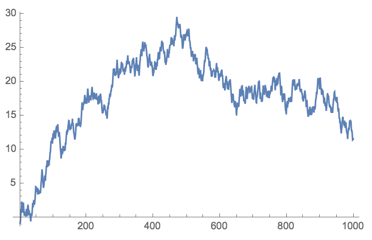
\includegraphics{todo.png}

\subsubsection{Unbalanced MNIST (DNN vs BNN vs DUE)}

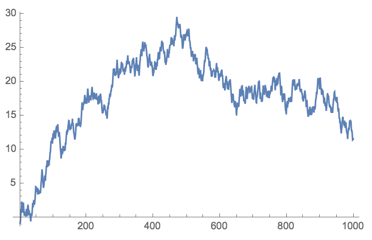
\includegraphics{todo.png}

\subsubsection{Repeated MNIST (DNN vs BNN vs DUE)}

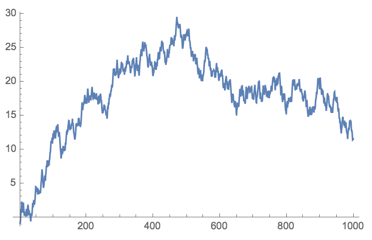
\includegraphics{todo.png}

\subsection{BALD}

\subsubsection{MNIST (BNN vs DUE)}

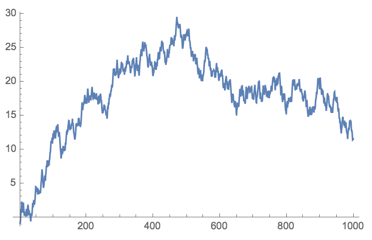
\includegraphics{todo.png}

\subsubsection{Unbalanced MNIST (BNN vs DUE)}

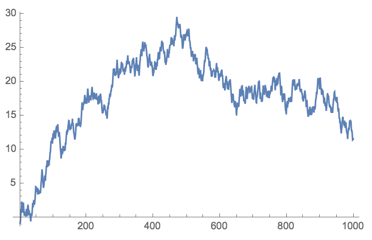
\includegraphics{todo.png}

\subsubsection{Repeated MNIST (BNN vs DUE)}

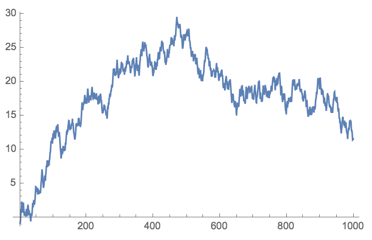
\includegraphics{todo.png}

\subsection{BatchBALD}

\subsubsection{MNIST (BNN vs DUE)}

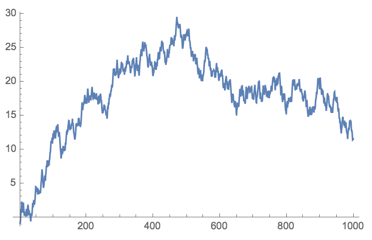
\includegraphics{todo.png}

\subsubsection{Unbalanced MNIST (BNN vs DUE)}

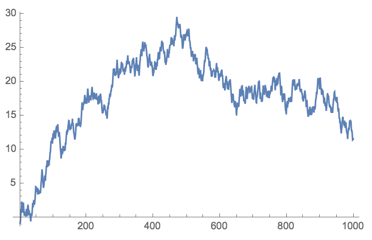
\includegraphics{todo.png}

\subsubsection{Repeated MNIST (BNN vs DUE)}

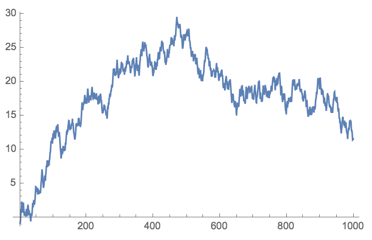
\includegraphics{todo.png}


\subsection{Predictive Entropy}

\subsubsection{MNIST (BNN vs DUE)}

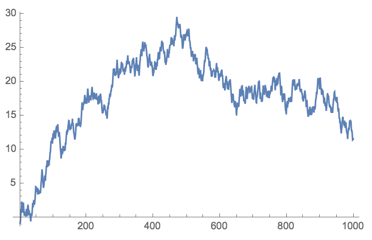
\includegraphics{todo.png}

\subsubsection{Unbalanced MNIST (BNN vs DUE)}

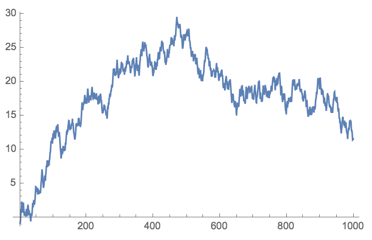
\includegraphics{todo.png}

\subsubsection{Repeated MNIST (BNN vs DUE)}

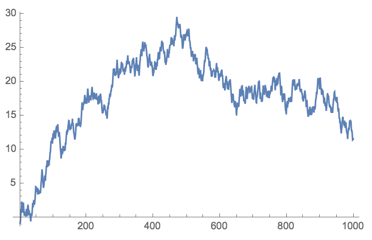
\includegraphics{todo.png}

\section{DUE}

To attempt to keep the experiments as comparible as possible, the feature extractor architecture used for DUE for this problem was the same architecture as the BNN with minimal modifications to satify the constraints of DUE. This primarily consisted of the additon of residual connections to the models, and the removal of the dropout layers.


\subsection{Training on small datasets}

Training a machine learning model on a small dataset can exaherbate many issues that we run into in machine learning. For example the models we have are even further over parameterised when we are operating in very small datasets.

While DUE has no problems in learning MNIST with more expressive models, eg more traditional ResNets. When using these the performance on very small datasets was reduced significantly, the performance of DUE on small subsets of MNIST was quite significatnly impacted.


\subsection{BALD}

\subsection{BatchBALD}

\subsection{Predictive Entropy}






\renewcommand{\bibname}{Bibliography}
\bibliographystyle{apacite}
\bibliography{Bibliography.bib}

\begin{appendices}
\chapter{Appendix}

\end{appendices}

\end{document}